\documentclass[article,nojss]{jss}\usepackage[]{graphicx}\usepackage[]{color}
% maxwidth is the original width if it is less than linewidth
% otherwise use linewidth (to make sure the graphics do not exceed the margin)
\makeatletter
\def\maxwidth{ %
  \ifdim\Gin@nat@width>\linewidth
    \linewidth
  \else
    \Gin@nat@width
  \fi
}
\makeatother


\usepackage{alltt}






%\usepackage{float}
%\usepackage{framed}
\usepackage{subcaption}
\renewcommand{\subfloat}[2][need a sub-caption]{ \subcaptionbox{#1}{#2} }
\usepackage{amsmath}
\usepackage[ruled,vlined]{algorithm2e}
\usepackage{listings}
\usepackage[shortcuts]{extdash}
\usepackage{booktabs}




%\addbibresource{paper2.bib}
\def\cov{{\text{COV}}}
\def\E{{\text{E}}}
\def\T{{\footnotesize{^{_{\sf T}}}}}
\setkeys{Gin}{width=0.45\textwidth}
\setcitestyle{square}




\newcommand{\class}[1]{`\code{#1}'}
\newcommand{\fct}[1]{\code{#1()}}







\author{Ruoyong Xu\\University of Toronto
   \And Patrick Brown\\University of Toronto
   \And Pierre L’Ecuyer\\University of Montr\'eal}
\Plainauthor{Ruoyong Xu, Patrick Brown, Pierre L’Ecuyer}


\title{A tool set for random number generation on GPUs in R}
\Plaintitle{}
\Shorttitle{}


\Abstract{
We introduce the \proglang{R} package \pkg{clrng} that leverages the \pkg{gpuR} package, and can generate random numbers on GPU by utilizing the \pkg{clRNG} (OpenCL) library. Parallel processing by graphics processing unit (GPU) can be used to speed up computationally intensive tasks, which when combined with \proglang{R}, it can largely improve \proglang{R}’s downsides in terms of slow speed, memory usage and computation mode.  There is currently no \proglang{R} package that does random number generation on GPU, while random number generation is critical in simulation-based statistical inference and modeling. \pkg{clrng} enables reproducible research by setting random streams on GPU and can thus accelerate several types of simulation and modelling. This package is portable and flexible, developers can use its random number generation kernel for various other purposes and applications. 
}


\Keywords{GPU, \pkg{clrng} package, parallel computing, \pkg{clRNG} library}
\Plainkeywords{GPU, clrng package, parallel computing, clRNG library}


\Address{
  Ruoyong Xu, Patrick Brown\\
  Department of Statistics\\
  University of Toronto\\
  700 University Ave., Toronto, ON M5G 1Z5, Canada\\
  E-mail: \email{ruoyong.xu@mail.utoronto.ca}, \email{patrick.brown@utoronto.ca}}


\Address{
  Pierre L’Ecuyer\\
  Department of Computer Science and Operations Research\\
  University of Montr\'eal\\
  Pavillon André-Aisenstadt 2920, chemin de la Tour Montréal QCH3T 1J4\\
  E-mail: \email{lecuyer@iro.umontreal.ca}}
\IfFileExists{upquote.sty}{\usepackage{upquote}}{}
\begin{document}
%\SweaveOpts{concordance=TRUE}





\section[Introduction]{Introduction}

% Why?
% 
% gpu massively parallel and relatively cheap, useful for stats
% there are gpu packages in R, gpuR
% no random numbers yet.  complicated to do on gpu, need multiple seeds becuase of parallel generation
% reproducability: need to save current state and restore

In recent years, parallel computing with \proglang{R} \citep{r2021} has become a very important topic and attracted lots of interest from researchers \citep[see][for a review]{eddelbuettel2021parallel}. Although \proglang{R} is one of the most popular statistical software with many advantages, it has drawbacks in memory usage and computation mode aspects \citep{zhao_2016}. To be more specific, (1) \proglang{R} requires all data to be loaded into the main memory (RAM) and thus can handle a very limited size of data; (2) \proglang{R} is a single-threaded program, it can not effectively use all the computing cores of multi-core processors. Parallel computing is the solution to these drawbacks, for an overview of current parallel computing approaches with \proglang{R}, see CRAN Task View by \citet{cran2021} at \url{https://cran.r-project.org/web/views/HighPerformanceComputing.html}. 

Graphics Processing Units (GPUs) have the potential to make important contribution to parallel computing with \proglang{R}. GPUs can perform thousands of tests simultaneously, which makes them powerful for doing massively parallel computing, and they are relatively cheap compared to multicore CPU's. Although there have been a number of \proglang{R} packages developed which provide some GPU capability, they inevitably come with some limitations. Packages such as \pkg{gputools}, \pkg{gpumatrix}, \pkg{cudaBayesreg}, \pkg{rpud} (available on github), are now no longer maintained, the popular \pkg{tensorflow} \citep{tensorflow1} package uses GPU via \proglang{Python}, which makes it difficult to include as a dependency for new \proglang{R} packages. All of these mentioned packages are restricted to \proglang{R} users with NVIDIA GPUs. \pkg{gpuR} \citep{gpur1} is the only \proglang{R} package with a convenient and flexible interface between \proglang{R} and GPUs, and it is compatible with many GPU devices. By utilizing the \pkg{ViennaCL} \citep*{rupp2016viennacl} library, it provides a bridge between \proglang{R} and non-proprietary GPUs through the \proglang{OpenCL} (Open Computing Language) backend, which when combined with \pkg{Rcpp} \citep{rcpp1} gives a building block for other \proglang{R} packages. 

Random number generation is critical in simulation-based statistical inference, machine learning and many other scientific fields. While most random number generators are sequential, the \proglang{R} packages \pkg{parallel}, \pkg{future} \citep*{future1.19.1} and \pkg{rlecuyer} \citep{sevcikova2015package} are able to generate random numbers in parallel on multicore CPUs. More specifically, \pkg{parallel} writes an interface for the \pkg{RngStreams}, a \proglang{\texttt{C++}} library by \cite{l2002object} which is based on a combined multiple-recursive generator (MRG) MRG32k3a. \pkg{future} and \pkg{rlecuyer} also uses the combined MRG algorithm for generating random numbers. For up-to-date review papers on the generation of random numbers on parallel devices, and GPUs in particular, see:  \cite{rLEC15a,rLEC17p,rLEC21a}.


The \pkg{clrng} package described here is currently the only \proglang{R} package that is able to generate random numbers on GPUs. Accomplishing this is complicated to do because each process must produce an independent sequence of random numbers, and in order to ensure reproducibility it should be possible to save and restore the current state of each stream of numbers at any point.  Here we introduce the \proglang{R} package \pkg{clrng} that leverages the \pkg{gpuR} package, and can generate random numbers on GPU by using the \proglang{clRNG} \citep{l2015clrng} library, and can thus accelerate several types of statistical simulation and modelling.



The remaining sections are organized as follows:
In Section 2, we introduce streams and the use of streams in work-items on a GPU device for generating uniform random numbers, and the usage of \fct{clrng::runif}.
In Section 3, we introduce two non-uniform RNGs in \pkg{clrng}, as examples for users to develop other RNGs of interest on GPUs in \proglang{R}.
In Section 4, we apply GPU-generated uniform random numbers in Monte Carlo simulation for Fisher’s exact test, we introduce how the random numbers are used and how the algorithm is parallelized and implemented on GPU. Then we provide two real data examples to demonstrate the function usage and its \proglang{R} performance.
Section 5, we show an useful application of normal random numbers on GPU, using them to simulate batches of Gaussian random surfaces with Mat\'ern covariance matrices simultaneously, the simulation also uses GPU-enabled functions from our another package \pkg{gpuBatchMatrix}.
Finally, the paper concludes with a short summary and a discussion in Section 6.






\section{Uniform random number generation} \label{}
Uniform random number generators (RNGs) are the foundation for simulating random numbers from all types of probability distributions. \cite{l2012random} summarized the usual two steps to generate a random variable in computational statistics: (1) generating independent and identically distributed (i.i.d.) uniform random variables on the interval $(0, 1)$, (2) applying transformations to these i.i.d. $U(0, 1)$ random variables to get samples from the desired distribution. \cite{l2012random} and \cite{robert2004random} present many general transformation methods for generating non-uniform random variables, for example, the most frequently used inverse transform method, the Box-Muller algorithm \citep{box1958note} for Gaussian random variable generation, and so on, which are all built on uniform random variables. %In the rest paper, ``RNG'' refers to uniform pseudo random number generator.


\proglang{clRNG} is an \proglang{OpenCL} library for uniform random number generation, it provides four different RNGs: the MRG31k3p, MRG32k3a, LFSR113, and Philox-4×32-10 generators. These four RNGs use different types of constructions. \pkg{clrng} package uses the MRG31k3p RNG, making it able to generate random numbers on GPUs. We choose MRG31k3p as the base generator for the following reasons:  the original \pkg{RNGStreams} package \citep{l2002object} was built with MRG32k3a, which was designed to be implemented in double precision, and not with 32-bit integers. The MRG31k3p generator was designed later, specifically for 32-bit integer arithmetic, so it runs faster on the 32-bit GPUs.  It is also faster than Philox-4×32-10 \citep{rLEC00b}. MRG31k3p was also statistically tested extensively and successfully, \cite[see][]{rLEC07b}.    




In what follows, we will illustrate how to create streams and how to use streams to generate uniform random numbers. 

%THE PROBLEM:  each process needs to be independent, there's a risk of overlap.  solution: streams.  mrg31kp3 a stream is a vector of three positive integers.  initial state is first stream, compute new streams sequentially.
\subsection{Creating streams}\label{createstreams}
Random number generation is more complicated when the RNG algorithm is run in parallel processes in \proglang{R}, there is a risk that the generated sequences of random numbers have correlation. \pkg{clrng} uses multiple distinct streams that are used in work-items that executes in parallel on a GPU device. A popular way of obtaining multiple streams is to take an RNG with a long period and cut the RNG's sequence into very long disjoint pieces of equal length $Z$, and use each piece as a separate stream. Creating a new stream amounts to computing its starting point. In general, a stream object contains three elements: the current state of the stream, the initial state of the stream (or seed), and the initial state of the current substream (by default it is equal to the seed). Streams are created sequentially in the way that whenever the user creates a new stream, the software automatically jumps ahead by Z steps to find its initial state, and the three states in the stream object are set to it. Each of these streams can also be partitioned into substreams with equally-spaced starting points \citep{l2002object, rLEC15a}.

In \proglang{clRNG} library, the MRG31k3p RNG's entire period of length approximately $2^{185}$ is divided into approximately $2^{51}$ non-overlapping streams of length $Z = 2^{134}$. Each stream can be further partitioned into substreams of length $2^{72}$, although this is not currently implemented in \pkg{clrng}. The state (and seed) of each stream is a vector of six 31-bit integers. This size of state is appropriate for having streams running in work-items on GPU cards, while providing a sufficient period length for most applications. The initial state of the first stream (also called ``initial seed for the package'' in \proglang{clRNG} and ``initial'' in \pkg{clrng}) for the MRG31k3p is by default $(12345, 12345, 12345, 12345, 12345, 12345)$. 


%The function \fct{clrngMrg31k3pCreateStreams} from \proglang{clRNG} creates streams on the host using the MRG31k3p RNG. If we want to use the streams in work-items on a GPU device, the streams have to be copied from the host to the global memory of the GPU device, and then each work-item copies the current states only of the streams to its private memory. 
\pkg{clrng} is able to create streams both on the host and on the GPU device. The \fct{createStreamsCpu} function does the former. The \proglang{R} output below creates 4 streams on the host.
%is an interface function of \fct{clrngMrg31k3pCreateStreams} that creates streams on host as \proglang{R} matrices, see the \proglang{R} output below, where we created 4 streams on the host using \fct{createStreamsCpu}, after transposing \code{myStreamsCpu}, each column of the matrix is a stream, creating streams on host makes it easy for us to view and check the streams behavior. Substreams are not created in \pkg{clrng} because currently we use one stream per work-item. 
\begin{CodeChunk}
\begin{CodeInput}
R> # creating streams on CPU
R> library("gpuR")
R> library("clrng")
R> myStreamsCpu <- createStreamsCpu(n = 4, initial = 12345)
R> t(myStreamsCpu)
\end{CodeInput}
\begin{CodeOutput}
##               [,1]       [,2]       [,3]       [,4]
## current.g1.1 12345  336690377  502033783  739421137
## current.g1.2 12345  597094797 1322587635 1475938232
## current.g1.3 12345 1245771585 1964121530  730262207
## current.g2.1 12345   85196284 1949818481 1630192198
## current.g2.2 12345  523477687 1607232546  324551134
## current.g2.3 12345 2094976052 1462898381  795289868
## initial.g1.1 12345  336690377  502033783  739421137
## initial.g1.2 12345  597094797 1322587635 1475938232
## initial.g1.3 12345 1245771585 1964121530  730262207
## initial.g2.1 12345   85196284 1949818481 1630192198
## initial.g2.2 12345  523477687 1607232546  324551134
## initial.g2.3 12345 2094976052 1462898381  795289868
\end{CodeOutput} 
\end{CodeChunk} 

\fct{createStreamsCpu} has two arguments:
\begin{itemize}
\itemsep0em 
  \item \code{n}: number of streams to create.
  \item \code{initial}: vector of length 6, recycled if shorter.
\end{itemize}
We move streams to the GPU by converting them to a `\code{vclMatrix}'. \fct{createStreamsGpu} creates streams directly on the GPU and returns a `\code{vclMatrix}', which makes it slightly more efficient when the number of streams is large. However, any data is lost when the \proglang{R} session is terminated. %\fct{createStreamsGpu} is adapted from the clrngMrg31k3pCreateStreams() and creates streams directly on a GPU device. Setting a seed same as the MRG31k3p default seed in \fct{createStreamsGpu}, we produce on device exactly the same streams as those created on host as follows. Notice that the code is just for showing \fct{createStreamsGpu} and \fct{createStreamsCpu} are \proglang{R} interface functions for \fct{clrngMrg31k3pCreateStreams} on GPU and CPU respectively, in practice it is not recommended to create a new stream that has the same initial seed as another existing stream in one simulation program.
\begin{CodeChunk}
\begin{CodeInput}
R> # creating streams on GPU
R> myStreamsGpu = vclMatrix(myStreamsCpu)
R> myStreamsGpu2 = createStreamsGpu(n = 4, initial = 12345)
\end{CodeInput} 
\end{CodeChunk} 


%also has the two arguments \code{n} and \code{initial}. \fct{createStreamsGpu} is similar to \code{.Random.seed} in \proglang{R}. By setting the RNG status with the \proglang{R} function \fct{set.seed}, we are able to repeat the sequence of random seeds, which is an important quality criteria of RNGs. Similarly in \fct{createStreamsGpu} and \fct{createStreamsCpu}, with the \code{initial} argument, we make the sequence of streams repeatable.






\subsection{Using streams to generate uniform random numbers}
The streams created sequentially are then used by the GPU's work-items to generate random numbers. In \pkg{clrng} each work-item takes one distinct stream to generate random numbers, so the number of streams should always be greater than the number of total work-items in use. The main part of the kernel (\proglang{OpenCL} functions for execution on the device) for generating uniform random numbers is shown in Listing \ref{lst:uniformkernel}. Users can set \code{verbose=2} in \fct{runif} to print out the kernels. Kernels are written in the \proglang{OpenCL C} language, in which \code{__kernel} declares a function as a kernel, pointer kernel arguments must be declared with an address space qualifier, for example \code{__global} and \code{__local}. Here the pointers to \code{streams} and to the output matrix \code{out} on the global memory are passed to the kernel as arguments. \code{Nrow} and \code{Ncol} represent row and column number of the matrix \code{out} respectively. \code{Npad} is the internal number of columns of \code{out}, \code{NpadStreams} is the internal number of columns of \code{streams} (these variables are defined in macros not shown here). \code{index} represents the position of a work-item when mapping it to a one-dimensional data structure. Each stream's current state is copied to the private memory of each work-item by the function \fct{streamsToPrivate}, in which \code{g1} and \code{g2} point to the first three and second three elements of stream states, respectively, and \code{startvalue} tells the starting position of the particular stream to be copied to the work-item. The function \fct{clrngMrg31k3pNextState} generates an uniform random integer named \code{temp} between 1 and 2147483647,  the value of \code{temp} is then scaled to be in the interval $(0,1)$ by multiplying it by a constant \code{mrg31k3p\_NORM\_cl}, which is defined to be $1/2147483648$ depending on the precision type. If to generate random integers, \code{temp} is not scaled. At the end of generating random numbers, streams are transferred back to global memory through the function \fct{streamsFromPrivate}.

\begin{lstlisting}[language=C,basicstyle=\small,label={lst:uniformkernel}]
__kernel void mrg31k3pMatrix(
  __global int* streams,
  __global float* out,
  int Nrow, int Ncol, int Npad){

int Drow, Dcol;
uint g1[3], g2[3];
float temp, fact = mrg31k3p_NORM_cl;

streamsToPrivate(streams,g1,g2,startvalue);

for(Drow=get_global_id(0); Drow < Nrow;
    Drow += get_global_size(0)){

    for(Dcol=get_global_id(1); DcolBlock < Ncol; 
        Dcol += get_global_size(1)){

        temp = fact * clrngMrg31k3pNextState(g1, g2);
        out[Drow * Npad + Dcol] = temp;

  }//Dcol
}//Drow

streamsFromPrivate(streams,g1,g2,startvalue);

}//kernel
\end{lstlisting}

%Figure \ref{fig:1} illustrates how this kernel executes in practice with a simple example. Suppose we have a $2 \times 4$ NDRange ((a) in Figure \ref{fig:1}) and want to create a $4 \times 6$ matrix ((b) in Figure \ref{fig:1}) of uniform random numbers. In each grid of (a) that represents a work-item, there are two rows of numbers, the number in the above row is the stream index (from 0 to 7), and a pair of numbers in the second row is the 2-dimensional global ID of the work-item. Each stream object is passed to each work-item. The number in a cell of the matrix corresponds to the stream index, it indicates which stream generates a random number for this matrix cell. %For example, stream 0 which is allocated in work-item $(0,0)$ generates a random number in matrix $(0,0)$ in the first iteration, then moves on to matrix $(0,2)$ and generates a random number there in the second iteration, in the third iteration it generates a random number in matrix $(0,4)$ and so on until it goes out of the matrix range in the next iteration.
% \begin{figure}[ht]
%     \centering
%     \subfloat[]{{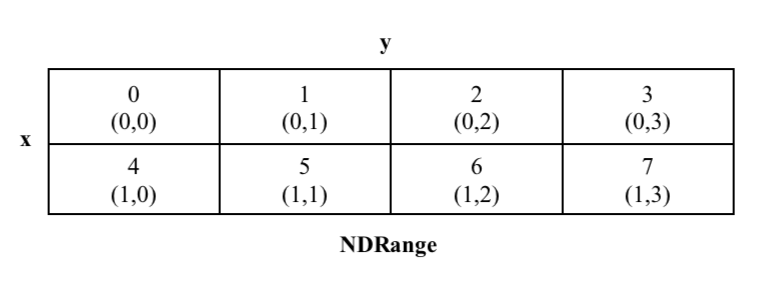
\includegraphics[width=8cm]{/home/ruoyong/diseasemapping/pkg/gpuRandom/inst/documents/paper1_2021_5/f1} }}
%     \qquad
%     \subfloat[]{{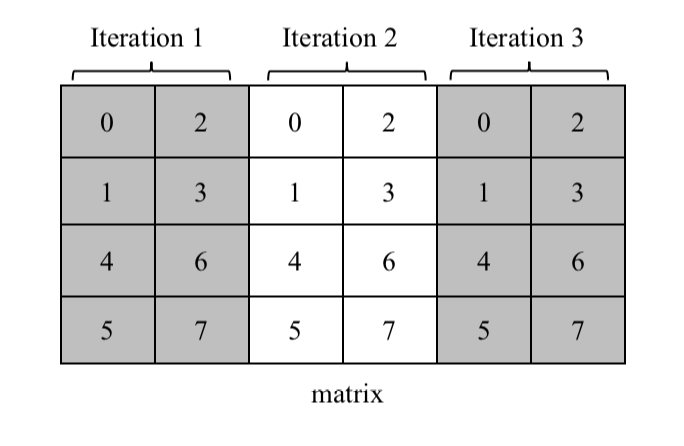
\includegraphics[width=8cm]{/home/ruoyong/diseasemapping/pkg/gpuRandom/inst/documents/paper1_2021_5/f2} }}
%     \caption{Using streams to produce a $4 \times 6$ matrix of random U(0,1) numbers. \label{fig:1}}
% \end{figure}

Now we use the streams created in section \ref{createstreams} to generate a vector of double-precision i.i.d. $U(0,1)$ random numbers with \fct{clrng::runif}. To view the generated random numbers, we need to convert them to \proglang{R} vectors or matrices, by doing this, the random numbers are moved from the global memory of the GPU device to the host.
\begin{CodeChunk}
\begin{CodeInput}
R> as.vector(clrng::runif(n = 6, streams = myStreamsGpu, Nglobal = c(2,
+    2)))
\end{CodeInput}
\begin{CodeOutput}
## [1] 0.735 0.842 0.614 0.216 0.110 0.870
\end{CodeOutput} 
\end{CodeChunk} 

The arguments of the \fct{clrng::runif} are described as follows:
\begin{itemize}
\itemsep0em 
  \item \code{n}: a vector of length 2 specifying the row and column number if to create a matrix, or a number specifying the length if to create a vector.
  \item \code{streams}: streams for random number generation.
  \item \code{Nglobal}: global index space. Default is set as $(64,8)$.
  \item \code{type}: ``double'' or ``float'' or ``integer'' format of generated random numbers.
  \item \code{verbose}: print extra information if $\text{verbose} > 1$. Default is FALSE.
\end{itemize}
%\fct{runif} returns the same sequence of random numbers because it uses the same streams \code{myStreamsGpu} and \code{myStreamsGpu2} here. 
Reusing \code{myStreamsGpu} will produce a vector different from \code{sim_1}. Because each time a random number is generated, the current state of the stream advances by one position. %Below shows the \code{myStreamsGpu} after it being used.

Unlike the objects created by \proglang{R}, by default they remain in the memory after a restart. Streams created on GPU does not remain in the memory when a new \proglang{R} session begins. However, we can save the streams on the CPU in a file using the \fct{saveRDS} function, and later recall the streams with the \fct{readRDS} function, in this way we can reproduce the exact same sequence of random numbers in simulations. Below is the code that saves streams to a data file called \code{streams_from_GPU.rds} on CPU and then load it back and transfer it to GPU.
\begin{CodeChunk}
\begin{CodeInput}
R> saveRDS(as.matrix(createStreamsGpu(n = 4)), "myStreams.rds")
R> # Load the streams object as streams_saved
R> streams_saved <- vclMatrix(readRDS("myStreams.rds"))
\end{CodeInput} 
\end{CodeChunk} 


%\subsection{Plot the uniform random numbers (now deleted?)}







\section{Some non-uniform random number generation}
\subsection{Normal random number generation}
We apply the Box-Muller transformation to $U(0,1)$ random numbers to generate standard normal random numbers. As shown in Algorithm \ref{algorithm1}, Box-Muller algorithm takes two independent, standard uniform random variables $U_1$ and $U_2$ and produces two independent, standard Gaussian random variables $X$ and $Y$, where $R$ and $\Theta$ are polar coordinate random variables. %The derivation basically uses transformation from Cartesian coordinates to polar coordinates to represent two independent, Normally distributed random variables. 
The Box-Muller algorithm is a very good choice for Gaussian transform on GPU compared to other transform methods \citep{howes2007efficient}, because this algorithm has no branching or looping, which are the things GPU is not good at. %but GPU is good at the high computational load of sine and cosine functions in the algorithm. 

\begin{algorithm}[ht] 
\SetAlgoLined
 1, Generate $U_1$, $U_2$ i.i.d. from $U (0,1)$ \;
 2, Define \begin{align*} 
& R = \sqrt{-2*\log U_1},\\
&  \Theta = 2\pi*U_2,\\
&  X=R*\cos(\Theta),\\
& Y=R*\sin(\Theta);\;\end{align*}
 3, Take $X$ and $Y$ as two independent draws from $N(0,1)$\;
 \caption{Box-Muller algorithm.}
 \label{algorithm1}
\end{algorithm}


Listing \ref{lst:normal} shows a fragment of the kernel that generates standard Gaussian random numbers. Aside from using local memory and the part that does the transformation, this kernel is the same with the kernel for generating uniform random numbers shown in Listing \ref{lst:uniformkernel}. If developers want to use other Gaussian transform methods, this kernel is easy to be adapted and incorporated in other \proglang{R} packages. The kernel executes over a 2-dimensional index space with $1 \times 2$ work-groups. \code{part[0]} and \code{part[1]} correspond to $R$ and $\Theta$ in the formulas respectively. \code{PI_2} is defined to be $\pi/2$. As the work-items in a work-group proceed at differing rates, \code{barrier(CLK_LOCAL_MEM_FENCE)} ensures correct ordering of memory operations to local memory, so that Gaussian random numbers $(X_1,Y_1), \dots, (X_n,Y_n)$ are generated in pairs correctly, errors such as $(X_n, Y_{(n-1)})$ or $(X_{(n-1)}, Y_{(n)})$ are avoided.
%

\begin{lstlisting}[language=C,basicstyle=\small,label={lst:normal},breaklines=true, escapeinside={(*@}{@*)}]
__kernel void mrg31k3pMatrix(
  __global int* streams,
  __global double* out,
  int Nrow, int Ncol, int Npad, int NpadStreams){

int Drow, Dcol;
uint g1[3], g2[3];
local double part[2];
int startvalue = (get_global_id(0) * get_global_size(1) + 
get_global_id(1)) * NpadStreams;

double sinOrCosPart1, addForSine = - get_local_id(1) * PI_2;
double temp, fact = mrg31k3p_NORM_cl;
if(get_local_id(1)){
  fact = TWOPI_mrg31k3p_NORM_cl;
}

streamsToPrivate(streams,g1,g2, startvalue);

for(Drow=get_global_id(0); Drow < Nrow;
    Drow += get_global_size(0)){

    for(Dcol=get_global_id(1); DcolBlock < Ncol; 
        Dcol += get_global_size(1)){
        
      temp = fact * clrngMrg31k3pNextState(g1, g2);
      part[get_local_id(1)] = temp;
      
      if(!get_local_id(1)) {
        part[0] = sqrt(-2.0*log(part[0]));
      }
      barrier(CLK_LOCAL_MEM_FENCE);
      
      // sine for local[1], cos for local[0]
      sinOrCosPart1 = cos(part[1] + addForSine);
      out[Drow * Npad + Dcol] = part[0]*sinOrCosPart1;

      barrier(CLK_LOCAL_MEM_FENCE);
  }//Dcol
}//Drow
streamsFromPrivate(streams,g1,g2,startvalue);
}//kernel
\end{lstlisting}

%We illustrate in Figure \ref{fig3} how this kernel executes in practice with the previous toy example: to create a $4 \times 6$ matrix of Gaussian random numbers using a $2 \times 4$ NDRange. %Each stream is copied to the private memory of each work-item. 
%Work-items are organized to be in 1 by 2 work-groups as the random numbers are generated in pairs using the Box-Muller method. The shading on the grids in the NDRange distinguishes work-groups. The numbers in the third row in each gird of NDRange represents the local index of each work-item. Each work-group generates a pair of Gaussian random numbers \code{(X,Y)} in each iteration, where work-item of `\code{get_local_id(1)}$=0$' generates the \code{X} of a pair, and work-item of `\code{get_local_id(1)}$=1$' generates the \code{Y} of a pair. %Here with the loop iterating over columns, the cells of matrix are filled from left to right, that is, in the first iteration, the 8 work-items generate random numbers in the leftmost two columns (8 cells) of the matrix simultaneously, the second iteration fills random numbers in the middle two columns of the matrix, and the third iteration fills the rest two columns of the matrix simultaneously. %Therefore, each work-item generates one Gaussian random number in each iteration, The matrix filling process is the same as that shown in Figure \ref{fig:1}. 

% \begin{figure}[ht]%
%     \centering
%     \subfloat[]{{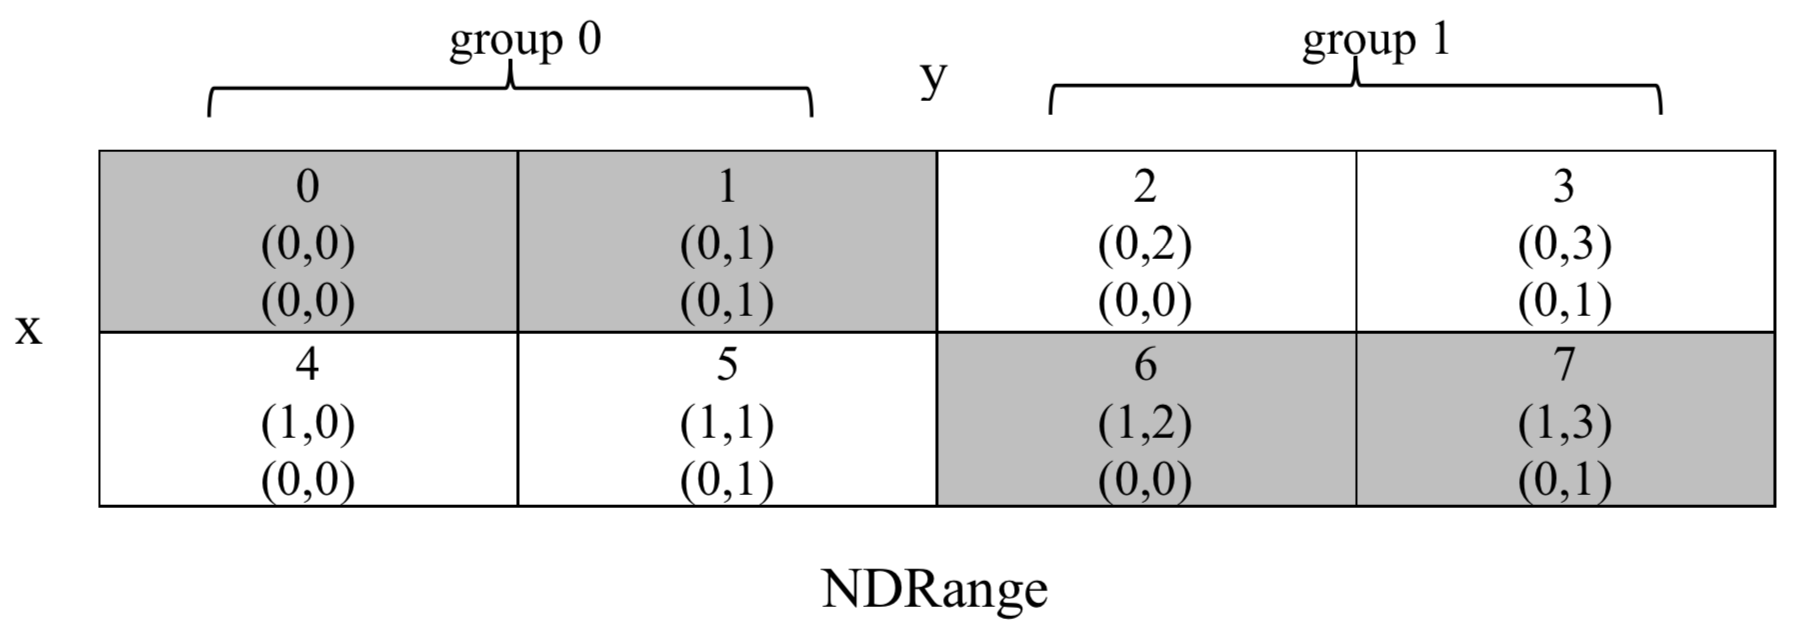
\includegraphics[width=8cm]{/home/ruoyong/diseasemapping/pkg/gpuRandom/inst/documents/paper1_2021_5/f3} }}%
%     \qquad
%     \subfloat[]{{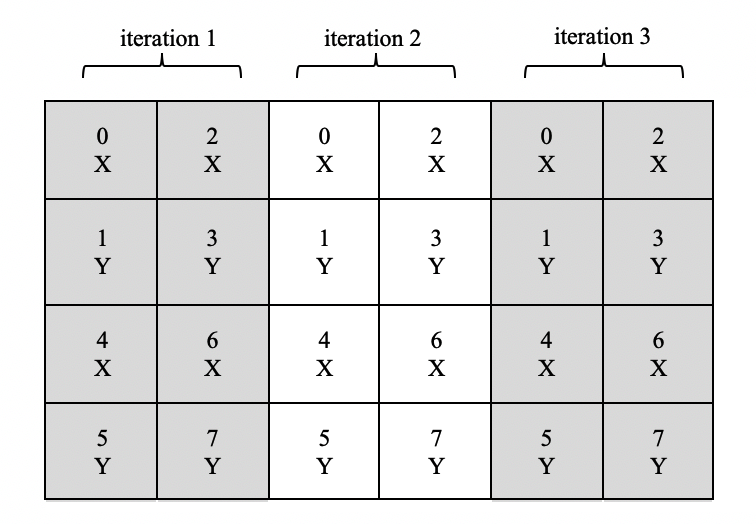
\includegraphics[width=8cm]{/home/ruoyong/diseasemapping/pkg/gpuRandom/inst/documents/paper1_2021_5/f4} }}%
%     \caption{Using streams to produce a $4 \times 6$ matrix of normal random numbers.}%
%     \label{fig3}
% \end{figure}
 

We generate a large-size matrix of 100 million double-precision Gaussian random numbers, and compare the run-time between using \fct{stats::rnorm} and \fct{clrng::rnorm}. The best performance we have seen using \fct{clrng::rnorm} is around 120 times faster with $512 \times 128$ work-items than using the \fct{stats::rnorm}. The difference in elapsed time becomes larger when matrix size goes larger.
\begin{CodeChunk}
\begin{CodeInput}
R> streams <- createStreamsGpu(n = 512 * 128)
R> system.time(clrng::rnorm(c(10000, 10000), streams = streams,
+    Nglobal = c(512, 128), type = "double"))
\end{CodeInput}
\begin{CodeOutput}
##    user  system elapsed 
##   0.043   0.004   0.047
\end{CodeOutput} 
\end{CodeChunk} 

\begin{CodeChunk}
\begin{CodeInput}
R> system.time(matrix(stats::rnorm(10000^2), 10000, 10000))
\end{CodeInput}
\begin{CodeOutput}
##    user  system elapsed 
##   6.700   0.828   7.526
\end{CodeOutput} 
\end{CodeChunk} 



\subsection{Exponential random number generation}
The exponential random variates are produced by applying the inverse transform method on i.i.d. $U(0,1)$ random numbers. The random variable $X \sim \text{Exponential}(\lambda)$ has cumulative distribution function $F_{X}(x)=1-e^{-\lambda x}$ for $x \geq 0$ and $\lambda > 0$. The inverse of $F_{X}(\cdot)$ is $F^{-1}_{X}(y)= -(1/ \lambda) \log (1-y)$, for $ 0 \leq y <1$. The kernel is not shown because it is mostly same as the kernel for uniform and normal random numbers, except for the part that does the inverse transform. %Developers can make use of our kernel for generating other types of random variables on GPU in \proglang{R}.

Below is an example that produces a matrix of Exponential random numbers with expectation equal to 1.
\begin{CodeChunk}
\begin{CodeInput}
R> r_matrix <- clrng::rexp(c(2, 4), rate = 1, Nglobal = c(2,
+    2), type = "double")
R> as.matrix(r_matrix)
\end{CodeInput}
\begin{CodeOutput}
##      [,1]  [,2]   [,3]  [,4]
## [1,] 1.48 1.916 1.0358 0.469
## [2,] 1.90 0.297 0.0868 0.161
\end{CodeOutput} 
\end{CodeChunk} 

The arguments of the \fct{clrng::rexp} are described as follows:
\begin{itemize}
\itemsep0em 
  \item \code{n}: a vector of length 2 specifying the row and column number if to create a matrix, or a number specifying the length if to create a vector.
  \item \code{streams}: streams. If missing, a stream with random initial state is supplied.
  \item \code{Nglobal}: global index space. Default is $(64,8)$.
  \item \code{type}: ``double'' or ``float'' format of generated random numbers.
  \item \code{verbose}: print extra information if $\text{verbose} > 1$. Default is FALSE.
\end{itemize}





\section{An application of uniform RNG: Fisher's simulation}
The GPU-generated random numbers can be applied in suitable statistical simulations to accelerate the performance.
One application of GPU-generated random numbers in \pkg{clrng} is Monte Carlo simulation for Fisher's exact test. Fisher’s exact test is applied for analyzing usually $2 \times 2$ contingency tables when one of the expected values in table is less than 5. Different from methods which rely on approximation, Fisher's exact test computes directly the probability of obtaining each possible combination of the data for the same row and column totals (marginal totals) as the observed table, and get the exact p-value by adding together all the probabilities of tables as extreme or more extreme than the one observed. However, when the observed table gets large in terms of sample size and table dimensions, the number of combinations of cell frequencies with the same marginal totals gets very large, \cite[][p. 23]{mehta2011ibm} shows a $5 \times 6$ observed table that has 1.6 billion possible tables. Calculating the exact P-values may lead to very long run-time and can sometimes exceed the memory limits of your computer. Hence, the option \code{simulate.p.value = TRUE} in \fct{stats::fisher.test} is provided, which enables computing p-values by Monte Carlo simulation for tables larger than 2 $\times$ 2. 

The test statistic calculated for each random table is $-\sum_{i,j}\log(n_{ij}!), i=(1,\dots, I), j=(1,\dots,J)$, (i.e., minus log-factorial of table), where $I$ and $J$ are the row and column number of the observed table. This test statistic can also be independently calculated for a table by \fct{clrng::logfactSum}. Given an observed table and a number of replicates $B$, the Monte Carlo simulation for Fisher's exact test does the following steps: 
\begin{enumerate}
\setlength\itemsep{0em}
  \item Calculate the test statistic for the observed table.
    \item In each iteration, simulate a random table with the same dimensions and marginal totals as the observed table using the \fct{rcont2} algorithm, compute and sometimes save the test statistic from the random table. 
    \item Count the number of iterations (\emph{Counts}) that have test statistics less or equal to the one from the observed table.
    \item Estimate p-value using $\frac{1 + \emph{Counts}}{B + 1}$.
\end{enumerate}

Step 1 and step 2-3 are done on a GPU with two kernels enqueued sequentially. For step 2, \fct{clrng::fisher.sim} adapted the function \fct{rcont2} used by \fct{stats::fisher.test} for constructing random two-way tables with given marginal totals. The algorithm \citep[see][]{patefield1981efficient} samples the entries row by row, one at a time, conditional on the values of the entries already sampled. The conditional probabilities for the possible values of the next entry are updated dynamically each time a new entry is sampled. Then this entry is sampled by standard inversion of the cumulative distribution function, using one $U(0,1)$ random number.  For an $I \times J$ table, this requires $(I-1)(J-1)$ random numbers (the last column and last row do not need to be sampled). Finally, one can compute the test statistic for this newly sampled table. On a GPU, this step can be replicated say $n$ times in parallel by creating $n$ distinct random streams and launching $n$ separate work-items. Each work-item takes a random stream as input, performs all of Step 2 and 3, and returns the value of the test statistic on the GPU. Computing the p-value on the CPU (Step 4) is then a trivial operation.  Step 2 of saving test statistics from the random tables is made optional, which can reduce the run-time. By the way, there are a lot of other more recent methods for sampling (larger) contingency tables, many of them use Markov Chain Monte Carlo, the use of streams and GPU would be quite different in that case. See for examples \citep{10.1214/13-AOS1131, KAYIBI2018298, dyer1997sampling}. Doing the \fct{fisher.sim} function on GPU opens up many possibilities for future work, the specific implementation we've done for the tables isn't necessarily the optimal one. 

The arguments of the \fct{clrng::fisher.sim} are described as follows:
\begin{itemize}
\setlength{\parskip}{0pt}
  \item \code{x}: a contingency table, a ``vclMatrix'' object.
  \item \code{N}: number of simulation runs.
  \item \code{streams}: streams.
  \item \code{type}: ``double'' or ``float'' of returned test statistics.
  \item \code{returnStatistics}: if TRUE, return all test statistics. 
  \item \code{Nglobal}: global index space. Default is set as $(64,16)$.
\end{itemize}
Users request $N$ number of replicates, while the actual number of replicates to be executed on GPU is larger (\code{ceiling(N/prod(Nglobal))*prod(Nglobal)}). We show the advantage of \fct{clrng::fisher.sim} by computing the p-values for two real data examples: one with a relatively big p-value and another with a very small p-value, and compare the run-time with using \fct{stats::fisher.test} for each of the data sets on two computers: one with a very good CPU and an ordinary GPU, the other is equipped with an excellent GPU and an ordinary CPU. The \proglang{R} outputs for testing on computer 2 is shown in the following. 


 
\subsection{Comparing run-time: Month data example}\label{fisher_month}
The 2-way contingency tables consist of selected data from the 2018 Natality public use data \citep{National2018} from the Centers for Disease Control and Prevention’s National Center for Health Statistics (NCHS), the 2018 natality data file may be downloaded at \url{https://www.cdc.gov/nchs/data_access/VitalStatsOnline.htm}. Table \ref{tab:month} is a $12 \times 12$ table that shows frequencies for congenital anomalies of the newborn by birth month in 2018 within the United States. The column variables of these two tables represent the twelve categories of congenital anomalies of the newborn: 1) Anencephaly; 2) Meningomyelocele/Spina bifida; 3) Cyanotic congenital heart disease; 4) Congenital diaphragmatic hernia; 5) Omphalocele; 6) Gastrochisis; 7) Limb reduction defect; 8) Cleft lip with or without cleft palate; 9) Cleft palate alone; 10) Down syndrome; 11) Suspected chromosomal disorder; and 12) Hypospadias. The first 5 rows of the table are displayed below.

 
\begin{table}

\caption{\label{tab:monthdata}Monthly birth anomaly data\label{tab:month}}
\centering
\begin{tabular}[t]{lrrrrrrrrrrrr}
\toprule
  & Ane & Men & Cya & Her & Omp & Gas & Lim & Cle & Pal & Dow & Chr & Hyp\\
\midrule
Jan & 29 & 55 & 172 & 46 & 39 & 73 & 48 & 183 & 77 & 103 & 102 & 174\\
Feb & 25 & 45 & 175 & 35 & 31 & 55 & 34 & 142 & 81 & 115 & 100 & 180\\
Mar & 31 & 48 & 182 & 41 & 47 & 72 & 40 & 200 & 86 & 90 & 96 & 180\\
Apr & 34 & 45 & 186 & 36 & 32 & 75 & 42 & 173 & 56 & 87 & 90 & 193\\
May & 33 & 40 & 187 & 46 & 24 & 80 & 35 & 180 & 75 & 91 & 100 & 197\\
Jun & 34 & 48 & 189 & 35 & 33 & 75 & 45 & 154 & 74 & 102 & 100 & 182\\
Jul & 26 & 43 & 198 & 34 & 21 & 74 & 36 & 179 & 79 & 86 & 92 & 193\\
Aug & 24 & 41 & 189 & 44 & 43 & 62 & 48 & 183 & 88 & 109 & 94 & 194\\
Sept & 34 & 44 & 147 & 40 & 37 & 66 & 36 & 158 & 73 & 112 & 103 & 196\\
Oct & 25 & 43 & 207 & 45 & 31 & 65 & 49 & 181 & 77 & 108 & 115 & 220\\
Nov & 36 & 55 & 188 & 39 & 39 & 62 & 43 & 144 & 68 & 98 & 79 & 173\\
Dec & 23 & 48 & 196 & 31 & 31 & 71 & 31 & 177 & 86 & 86 & 73 & 156\\
\bottomrule
\end{tabular}
\end{table}



\begin{CodeChunk}
\begin{CodeInput}
R> streams <- createStreamsGpu(n = 256 * 64, initial = 666)
R> month_gpu <- vclMatrix(month, type = "integer")
R> system.time(result_month <- clrng::fisher.sim(month_gpu, 1e+06,
+    streams = streams, type = "double", returnStatistics = TRUE,
+    Nglobal = c(256, 64)))
\end{CodeInput}
\begin{CodeOutput}
##    user  system elapsed 
##   0.322   0.011   0.333
\end{CodeOutput}
\begin{CodeInput}
R> result_month$threshold
\end{CodeInput}
\begin{CodeOutput}
## [1] -47955
\end{CodeOutput}
\begin{CodeInput}
R> result_month$simNum
\end{CodeInput}
\begin{CodeOutput}
## [1] 1015808
\end{CodeOutput}
\begin{CodeInput}
R> result_month$counts
\end{CodeInput}
\begin{CodeOutput}
## [1] 410825
\end{CodeOutput}
\begin{CodeInput}
R> result_month$p.value
\end{CodeInput}
\begin{CodeOutput}
## [1] 0.404
\end{CodeOutput} 
\end{CodeChunk} 

We got 410825 cases whose test statistics are below the observed threshold based on an actual number of 1015808 simulations, so the p-value from \fct{clrng::fisher.sim} for this table is about 0.40443, which is close enough to the p-value from \fct{stats::fisher.test}. \fct{clrng::fisher.sim} takes about 0.31 seconds, \pkg{clrng} accounts for 2.17\% of the elapsed time on CPU. 

 
\begin{CodeChunk}
\begin{CodeInput}
R> # using CPU
R> system.time(result_monthcpu <- stats::fisher.test(month, simulate.p.value = TRUE,
+    B = 1e+06))
\end{CodeInput}
\begin{CodeOutput}
##    user  system elapsed 
##  14.455   0.028  14.478
\end{CodeOutput}
\begin{CodeInput}
R> result_monthcpu$p.value
\end{CodeInput}
\begin{CodeOutput}
## [1] 0.403
\end{CodeOutput} 
\end{CodeChunk} 




\subsection{Comparing run-time: Week data example}\label{fisher_week}
Table \ref{tab:week} is a $7 \times 12$ table shows frequencies for congenital anomalies of the newborn by birth day of week in 2018 within the United States. 


\begin{table}

\caption{\label{tab:weekdata}Day-of-week birth anomaly data\label{tab:week}}
\centering
\begin{tabular}[t]{lrrrrrrrrrrrr}
\toprule
  & Ane & Men & Cya & Her & Omp & Gas & Lim & Cle & Pal & Dow & Chr & Hyp\\
\midrule
Mon & 30 & 34 & 173 & 37 & 23 & 80 & 49 & 191 & 83 & 122 & 109 & 216\\
Tue & 60 & 121 & 383 & 80 & 83 & 131 & 71 & 349 & 146 & 164 & 168 & 352\\
Wed & 51 & 106 & 417 & 92 & 73 & 145 & 72 & 333 & 136 & 179 & 196 & 351\\
Thu & 60 & 86 & 362 & 69 & 74 & 120 & 85 & 326 & 132 & 220 & 187 & 359\\
Fri & 52 & 94 & 347 & 87 & 59 & 123 & 68 & 323 & 145 & 170 & 166 & 345\\
Sat & 52 & 63 & 323 & 67 & 64 & 135 & 73 & 316 & 170 & 189 & 188 & 357\\
Sun & 49 & 51 & 211 & 40 & 32 & 96 & 69 & 216 & 108 & 143 & 130 & 258\\
\bottomrule
\end{tabular}
\end{table}




\begin{CodeChunk}
\begin{CodeInput}
R> week_GPU <- gpuR::vclMatrix(week, type = "integer")
R> system.time(result_week <- clrng::fisher.sim(week_GPU, 1e+07,
+    streams = streams, type = "double", returnStatistics = TRUE,
+    Nglobal = c(256, 64)))
\end{CodeInput}
\begin{CodeOutput}
##    user  system elapsed 
##   1.930   0.021   1.950
\end{CodeOutput}
\begin{CodeInput}
R> result_week$threshold
\end{CodeInput}
\begin{CodeOutput}
## [1] -54990
\end{CodeOutput}
\begin{CodeInput}
R> result_week$simNum
\end{CodeInput}
\begin{CodeOutput}
## [1] 1e+07
\end{CodeOutput}
\begin{CodeInput}
R> result_week$counts
\end{CodeInput}
\begin{CodeOutput}
## [1] 1193
\end{CodeOutput}
\begin{CodeInput}
R> result_week$p.value
\end{CodeInput}
\begin{CodeOutput}
## [1] 0.000119
\end{CodeOutput} 
\end{CodeChunk} 

The ``week'' table has a much smaller p-value: around 0.0001249672, which should require a larger number of simulations to get a more accurate p-value. With more than ten million simulations, we get 1205 cases and a p-value around 0.000120472 by \fct{fisher.sim}. \fct{stats::fisher.test} takes 91.6 seconds, while \fct{fisher.sim} takes about 4.282 seconds, the elapsed time is decreased to about 4.67\% of the time taken on CPU. 


\begin{CodeChunk}
\begin{CodeInput}
R> # using CPU
R> system.time(result_weekcpu <- fisher.test(week, simulate.p.value = TRUE,
+    B = 10010624))
\end{CodeInput}
\begin{CodeOutput}
##    user  system elapsed 
##  89.968   0.096  90.031
\end{CodeOutput}
\begin{CodeInput}
R> result_weekcpu$p.value
\end{CodeInput}
\begin{CodeOutput}
## [1] 0.000132
\end{CodeOutput} 
\end{CodeChunk} 



\subsection{A summary of the results}
We summarized the comparison results in the table \ref{tab:summary} and plot the test statistics in Figure %\ref{fig4}.
\begin{table}

\caption{\label{tab:summarycompare}Summary of comparions of Fisher's test simulation on different devices. Computer 1 is equipped with CPU Intel Xenon W-2145 3.7Ghz and AMD Radeon VII. Computer 2 is equipped with VCPU Intel Xenon Skylake 2.5Ghz and VGPU Nvidia Tesla V100.\label{tab:summary}}
\centering
\begin{tabular}[t]{l|l|l|l|l|l}
\hline
\multicolumn{1}{c|}{ } & \multicolumn{2}{c|}{Computer 1} & \multicolumn{2}{c|}{Computer 2} & \multicolumn{1}{c}{ } \\
\cline{2-3} \cline{4-5}
B & Intel 2.5ghz & AMD Radeon & Intel 3.7ghz & NVIDIA V100 & Data\\
\hline
\multicolumn{6}{l}{\textbf{P-value}}\\
\hline
\hspace{1em}1M & 0.403804 & 0.403507 & 0.4035606 & 0.403507 & month\\
\hline
\hspace{1em}10M & 0.0001251 & 0.0001274 & 0.0001202 & 0.0001274 & week\\
\hline
\multicolumn{6}{l}{\textbf{Run-time}}\\
\hline
\hspace{1em}1M & 10.74 & 2.28 & 15 & 0.72 & month\\
\hline
\hspace{1em}10M & 63.24 & 10.82 & 91.58 & 4.18 & week\\
\hline
\end{tabular}
\end{table}





\begin{figure}

{\centering \subfloat[Month data\label{fig:fighistMonth-1}]{\includegraphics[width=0.47\textwidth]{Figures/GfighistMonth-1} }
\subfloat[week data\label{fig:fighistMonth-2}]{\includegraphics[width=0.47\textwidth]{Figures/GfighistMonth-2} }

}

\caption[Approximate sampling distributions of the test statistics from the two examples Month and Week]{Approximate sampling distributions of the test statistics from the two examples Month and Week. The test statistic values of the observed tables are marked with a blue line on each plot.}\label{fig:fighistMonth}
\end{figure}









\section{An application of normal RNG: Gaussian surface simulation} 
Given a parameter space $X$, a random field $U$ on $X$ is a collection of random variables $\{U_x :x\in X\}$. A Gaussian random field is a random field with the property that for any positive integer $n$ and any set of locations $x_1,\dots,x_n \in X$, the joint distribution of $U=(U_{x_1},\dots,U_{x_n})$ is multivariate Gaussian. The expectation of $U$ and covariance function $\Sigma$ completely determine the distribution of $U$, where 
\begin{gather*} 
U = [U(x_1), \ldots, U(x_n)]^\top \sim \text{MVN}(0, \Sigma) \\
\Sigma_{ij} = \cov[ U(x_i),U(x_j) ] = \sigma^2 \frac{2^{\kappa-1}}{\Gamma(\kappa)} \left(\sqrt{8\kappa} \frac{|x_i = x_j|}{\phi}\right)^\kappa  K_\kappa\left(\sqrt{8\kappa}  \frac{|x_i = x_j|}{\phi}\right).
\end{gather*}
The common choice for the covariance function $\Sigma$ is the Mat\'ern covariance function \citep{matern1960spatial}. The Mat\'ern covariance between $U(x_i)$ and $U(x_j)$ takes the above form.
%$d =\|x-x'\|$ is the Euclidean distance between two spatial points, 
$\sigma^2$ the variance of the random field $U$.
$\Gamma(\cdot)$ is the standard gamma function,  $\phi$ is the range parameter or scale parameter with the dimension of distance, it controls the rate of decay of the correlation as distance increases. $K_\kappa(\cdot)$ is the modified Bessel function of the second kind with order $\kappa$, $\kappa$ is the shape parameter which determines the smoothness of $U(x)$, specifically, $U(x)$ is $m$ times mean-square differentiable if and only if $\kappa > m$. %(For $\kappa=0.5$, the Mat\'ern covariance function reduces to the exponential covariance function $\sigma^2*\exp(-d/\phi)$, when $\kappa \rightarrow \infty$, $\Sigma(d) \rightarrow \sigma^2*\exp{-(\|d\|/\phi)^2}$, which is called the Gaussian covariance.)  
There are several alternative parameterisations of Mat\'ern covariance functions in literatures  \citep[see][]{haskard2007anisotropic}. In \pkg{clrng}, we use the above form for computing Mat\'ern covariance.


%Due to the importance of Gaussian random field, there are a large amount of studies devoted to Gaussian random field generation techniques. 
\cite{LiuandLi2019} gives a comprehensive review on 7 popular methods for Gaussian random field generation, %which are the turning bands method \citep{matheron_1973}, spectral method \citep{Meja1974OnTS,1972JSV}, matrix decomposition method \citep{davis1987}, Karhunen-Lo\'eve expansion \citep{LoeveM:1978}, moving average method \citep{journel1974, oliver1995moving}, sequential simulation \citep{johnson1987multivariate, gomez1993joint, pebesma2004multivariable}, and local average subdivision \citep{fenton1990simulation}. 
all of these methods except matrix decomposition method, are approximations and has specific requirements on the type of grid or covariance functions. The matrix decomposition method is exact, it works for all covariance functions and can generate random field on all types of grids. Other \proglang{R} packages that offer simulation of Gaussian random fields like \pkg{geoR} \citep{geoR2001}, does not work for large number of locations; the \pkg{RandomFields} \citep{RandomFields2015,RandomFields2020} package can use different methods for simulation of Gaussian fields, among which the (modified) circulant embedding method \citep{Dietrich1997FastAE} for covariance matrix decomposition is also an exact method (need to confirm???), however, it works only for isotropic Gaussian fields and on rectangular grids. \pkg{clrng} does exact simulation of exact Gaussian fields on the GPU as it relies on the matrix decomposition method. The implementation of this method is as follows.


Suppose $U=(U_1, U_2, \dots, U_n)$ is a Gaussian random field with mean $\mu$ and covariance matrix $\Sigma$, without loss of generality, we assume mean value zero $(\mu = 0)$. Since covariance matrix $\Sigma$ is symmetric and positive-definite, we can take Cholesky decomposition of $\Sigma$, then we can simulate random samples from $U$ using Algorithm \ref{algorithm2},

\begin{algorithm}[ht]
\SetAlgoLined
 1, Calculate the covariance matrix $\Sigma$ between locations\;
 2, Compute the Cholesky decomposition of $\Sigma = L \cdot D \cdot L^\top$, $L$ is the lower unit triangular matrix, $D$ is a diagonal matrix\;
 3, Generate on GPU a random matrix $Z=(Z_1, Z_2, \dots, Z_n) \sim \text{MVN}(0,I_n)$, where $I_n$ is a $n \times n$ identity matrix\;
 4, Compute the random samples from $U$ in batches using $U = L \cdot D^{\frac{1}{2}} \cdot Z$ \;
 \caption{Gaussian random fields simulation using covariance matrix decomposition method.}
 \label{algorithm2}
\end{algorithm}

% $U=L*D^{1/2}*Z$, where 
% \begin{itemize}
% \itemsep0em 
% \item $L$ is the lower unit triangular matrix in Cholesky decomposition of $\Sigma = L*D*L^\top$,
% \item $D$ is a diagonal matrix.
% \item $Z=(Z_1, Z_2, \dots, Z_n) \sim \text{MVN}(0,I_n)$, where $I_n$ is a $n \times n$ identity matrix.
% \end{itemize}
The matrix decomposition method is straightforward to implement. However, when a large number of locations $n$ is involved, the cost of Cholesky decomposition of the covariance matrix is $\mathcal{O}(n^3)$,  and the cost of matrix-vector multiplication $L*Z$ to generate the random field $U$ is $\mathcal{O}(n^2)$ \citep{LiuandLi2019}.  Our another \proglang{R} package \pkg{gpuBatchMatrix} is able to compute batches of Mat\'ern covariance matrices in parallel, and do Cholesky decomposition and matrix-matrix multiplication in batches in parallel on GPU. The following shows an example, in which we simulate on GPU 10 Gaussian random fields of mat\'ern covariance at one time with 5 sets of parameters, by taking advantage of the GPU-capabilities provided by \pkg{clrng} and \pkg{gpuBatchMatrix} together.
%\pkg{clrng} package not only does the matrices decomposition (Cholesky decomposition and matrix-vector multiplication) in parallel, but also computes the covariance matrices in parallel on GPU. 

\subsection{Simulating Gaussian random fields with Mat\'ern covariances}
\begin{CodeChunk}
\begin{CodeInput}
R> library("gpuR")
R> library("clrng")
R> library("gpuBatchMatrix")
R> library("geostatsp")
\end{CodeInput} 
\end{CodeChunk} 

Step 1, set up a $60 \times 80$ raster and coordinates on the raster, convert the matrix of coordinates \code{coordsSp@coords} to a ``vclMatrix'' object for later use.
\begin{CodeChunk}
\begin{CodeInput}
R> NlocalCache = 1000
R> Nglobal = c(128, 64, 2)
R> Nlocal = c(4, 2, 2)
R> theType = "double"
\end{CodeInput} 
\end{CodeChunk} 


\begin{CodeChunk}
\begin{CodeInput}
R> data("swissRain", package = "geostatsp")
R> myRaster = geostatsp::squareRaster(swissBorder, 80)
R> myRaster
\end{CodeInput}
\begin{CodeOutput}
## class      : RasterLayer 
## dimensions : 51, 80, 4080  (nrow, ncol, ncell)
## resolution : 4358, 4358  (x, y)
## extent     : 2485351, 2833996, 1075013, 1297275  (xmin, xmax, ymin, ymax)
## crs        : +proj=somerc +lat_0=46.9524055555556 +lon_0=7.43958333333333 +k_0=1 +x_0=2600000 +y_0=1200000 +ellps=GRS80 +units=m +no_defs
\end{CodeOutput} 
\end{CodeChunk} 

Step 2, create 5 parameter sets as a small example, in practical studies, there can be hundreds or thousands of parameter sets. Then, convert the matrix of parameters to a ``vclMatrix'' for later use by \fct{gpuBatchMatrix::maternGpuParam}.

\begin{CodeChunk}
\begin{CodeInput}
R> params
\end{CodeInput}
\begin{CodeOutput}
##      shape range variance nugget anisoRatio
## [1,]  1.25 50000      1.5      0          1
## [2,]  2.15 60000      2.0      0          4
## [3,]  0.60 30000      2.0      0          2
## [4,]  3.00 30000      2.0      0          2
##      anisoAngleRadians
## [1,]             0.000
## [2,]             0.449
## [3,]             0.449
## [4,]             0.449
\end{CodeOutput}
\begin{CodeInput}
R> # paramsGpu =
R> # gpuBatchMatrix::maternGpuParam(myParamsBatch,
R> # type=theType)
\end{CodeInput} 
\end{CodeChunk} 

Step 3, compute Mat\'ern covariance matrices using \fct{gpuBatchMatrix::maternBatch}, the returned Mat\'ern covariance matrices %$\Sigma_1, \Sigma_2, \dots, \Sigma_5$ correspond to the 5 parameter sets respectively, the matrices 
are each of size $4800 \times 4800$ and are stacked by row in the output \code{maternCov}. 
\begin{CodeChunk}
\begin{CodeInput}
R> # maternCov = vclMatrix(0,
R> # nrow(paramsGpu)*nrow(coordsGpu),
R> # nrow(coordsGpu),type=theType)
R> maternCov = gpuBatchMatrix::maternBatch(params, myRaster,
+    Nglobal = c(128, 64), Nlocal = c(16, 4))
R> dim(maternCov)
\end{CodeInput}
\begin{CodeOutput}
## [1] 16320  4080
\end{CodeOutput} 
\end{CodeChunk} 

Step 4, the first argument \code{A} in \fct{gpuBatchMatrix::cholBatch} specifies the object to take Cholesky decomposition. Computed unit lower triangular matrices $L_i$'s are stacked by row and stored in \code{maternCov}. Each row of \code{diagMat} stores the diagonal values of each $D_i$, for example, if each batch $\Sigma_i$ is of size $n \times n$, then each batch $L_i$ is $n \times n$, and each batch $D_i$ is $1 \times n$.
\begin{CodeChunk}
\begin{CodeInput}
R> diagMat = gpuBatchMatrix::cholBatch(maternCov, Nglobal = c(128,
+    8), Nlocal = c(32, 8))
\end{CodeInput} 
\end{CodeChunk} 

\begin{gather}
\begin{bmatrix} \Sigma_{1} \\ \Sigma_2 \\ \Sigma_3 \\ \vdots
\end{bmatrix}
 \rightarrow
 \begin{bmatrix}
  L_{1} \\ L_{2} \\L_{3} \\ \vdots
  \end{bmatrix} \text{and}
  \begin{bmatrix}
  D_{1} \\ D_{2} \\D_{3} \\ \vdots
  \end{bmatrix}
\end{gather}
Step 5, generate 2 standard Gaussian random vectors \code{zmatGpu}$=(Z_1, Z_2)$ using \fct{clrng::rnorm}, in which \code{c(nrow(materCov),2)} specifies the number of rows and columns of \code{zmatGpu}.
\begin{CodeChunk}
\begin{CodeInput}
R> streamsGpu <- createStreamsGpu(n = 128 * 64)
\end{CodeInput} 
\end{CodeChunk} 

\begin{CodeChunk}
\begin{CodeInput}
R> zmatGpu = clrng::rnorm(c(nrow(maternCov), 2), streams = streamsGpu,
+    Nglobal = c(128, 64), type = theType)
\end{CodeInput} 
\end{CodeChunk} 

Step 6, use \fct{gpuBatchMatrix::multiplyLowerDiagonalBatch} to compute $U = L * D^{(1/2)}* Z$ in batches, see the following illustration. \code{simMat} is the output matrix for $U$, \code{maternCov}, \code{diagMat}, and \code{zmatGpu} correspond to the matrices of $L$, $D$ and $Z=(Z_1, Z_2)$ respectively.
\begin{CodeChunk}
\begin{CodeInput}
R> simMat = vclMatrix(0, nrow(zmatGpu), ncol(zmatGpu), type = gpuR::typeof(zmatGpu))
R> gpuBatchMatrix::multiplyLowerDiagonalBatch(output = simMat,
+    L = maternCov, D = diagMat, B = zmatGpu, diagIsOne = TRUE,
+    transformD = "sqrt", Nglobal, Nlocal, NlocalCache)
\end{CodeInput} 
\end{CodeChunk} 

\begin{gather}
 \begin{bmatrix}  L_{1} \\ L_{2} \\L_{3} \\ \vdots
 \end{bmatrix} 
 *
  \begin{bmatrix}
   D_{1} \\ D_{2} \\D_{3} \\ \vdots
   \end{bmatrix} 
   *
   \begin{bmatrix}
   Z_{11} & Z_{12}
   \end{bmatrix}
  =
 \begin{bmatrix}
   L_1D_1Z_{11} & L_1D_1Z_{12} \\
   L_2D_2Z_{11} & L_2D_2Z_{12} \\
   L_3D_3Z_{11} & L_3D_3Z_{12} \\
   \vdots  &   \vdots
  \end{bmatrix}
\end{gather}
Step 7, Finally, plot the 10 realizations.
\begin{CodeChunk}
\begin{CodeInput}
R> simRaster = raster::brick(myRaster, nl = ncol(simMat) * nrow(params))
R> values(simRaster) = as.vector(as.matrix(simMat))
\end{CodeInput} 
\end{CodeChunk} 




\begin{figure}
\subfloat[parameter 1, simuation 1\label{fig:maternplot-1}]{\includegraphics[width=0.47\textwidth]{Figures/Gmaternplot-1} }
\subfloat[parameter 2, simuation 1\label{fig:maternplot-2}]{\includegraphics[width=0.47\textwidth]{Figures/Gmaternplot-2} }
\subfloat[parameter 3, simuation 1\label{fig:maternplot-3}]{\includegraphics[width=0.47\textwidth]{Figures/Gmaternplot-3} }
\subfloat[parameter 4, simuation 1\label{fig:maternplot-4}]{\includegraphics[width=0.47\textwidth]{Figures/Gmaternplot-4} }
\subfloat[parameter 1, simuation 2\label{fig:maternplot-5}]{\includegraphics[width=0.47\textwidth]{Figures/Gmaternplot-5} }
\subfloat[parameter 2, simuation 2\label{fig:maternplot-6}]{\includegraphics[width=0.47\textwidth]{Figures/Gmaternplot-6} }
\subfloat[parameter 3, simuation 2\label{fig:maternplot-7}]{\includegraphics[width=0.47\textwidth]{Figures/Gmaternplot-7} }
\subfloat[parameter 4, simuation 2\label{fig:maternplot-8}]{\includegraphics[width=0.47\textwidth]{Figures/Gmaternplot-8} }\caption[Simulated Gaussian random fields]{Simulated Gaussian random fields}\label{fig:maternplot}
\end{figure}








\section{Discussion}
The package \pkg{clrng} has been created to make GPU-generated uniform and normal random numbers accessible for \proglang{R} users, it enables reproducible research in simulations by setting seeds in streams on GPU. We further applied the GPU-generated random numbers in suitable statistical simulations, such as the Monte Carlo simulation for Fisher’s exact test, and (exact) Gaussian spatial surfaces simulation, for which we are able to calculate quantiles for the normal distribution, compute mat\'ern covariance matrices, do Cholesky decomposition and matrix multiplication in batches on GPU. Most of these functions uses local memory on GPU. Comparison of performance between using \pkg{clrng} and using classic \proglang{R} on CPU for some real data examples has demonstrated significant improvement in execution time. 

By leveraging the \pkg{gpuR} package, \pkg{clrng} provides a user-friendly interface that bridges \proglang{R} and \proglang{OpenCL}, users can use the facilities in our package without the need to know the complex \proglang{OpenCL} or even the \proglang{\texttt{C++}} code.  \pkg{clrng} is portable as its backend \proglang{OpenCL} supports multiple types of processors, and it is also flexible as its kernels can be incorporated or reconstructed in other \proglang{R} packages for other applications. 

%One of the main difficulties in developing the package is bug fixes and uncertain software behaviors. Error messages are often vague and it is time-consuming to locate the error within the backend \proglang{C} program. The usual steps that we take to debug is commenting out some parts of codes and then recompile many times until we find the problem, or printing out flag messages in several places in the code to find out where the program stops at due to error. 

\pkg{clrng} is limited by the number and type of \proglang{OpenCL} RNGs used and the features of the \pkg{gpuR} package, as it depends upon the \pkg{gpuR} package, if developers wants to use our package to do something that's not supported in \pkg{gpuR}, for example ``sparse'' class objects, they would have to write \proglang{OpenCL} code to implement it.

Future work on \pkg{clrng} package could be: (1) Explore other RNGs, for example the MRG32k3a, LFSR113, and Philox-4×32-10 generators in \proglang{clRNG} library, and compare the \proglang{R} performance between using different GPU RNGs. (2) Now that the package can do Cholesky decomposition and matrix multiplication in batches on GPU, which is a motivation for us to work on parallel likelihood evaluations on GPU for Gaussian spatial models in the next step. (3) Create a ``sparse'' matrix class on GPU and use it for simulating Gaussian random fields with sparse correlation structures such as the Gaussian Markov random fields.





\bibliography{paper1}




\newpage












\begin{appendix}

\end{appendix}


\end{document}




